\documentclass[12pt]{article} % Clase de documento
\usepackage[utf8]{inputenc}
\usepackage{csquotes} % Recommended for biblatex
\usepackage{tocbasic}  % Estilos de la TOC
\usepackage[spanish]{babel}
\usepackage{lmodern} % Soluciona problemas de sustitución de tamaño de fuente
\usepackage{amsfonts} % Para símbolos matemáticos
\usepackage{graphicx} % Para imágenes
\usepackage{hyperref} % Para enlaces y referencias en el índice
\usepackage{titling}  % Para personalizar la portada
\usepackage{geometry} % Márgenes
\usepackage{titlesec} % Para personalizar títulos
\usepackage[backend=bibtex,style=ieee]{biblatex}
\addbibresource{bibliografia.bib} % Archivo de bibliografía
\usepackage{amsmath} % Para ecuaciones matemáticas
% Personalización del título en la portada
\newcommand{\customtitlefont}{\fontsize{40pt}{42pt}\selectfont\bfseries} % Cambia el tamaño y estilo

\geometry{a4paper, margin=2.5cm}

\title{Detección de cáncer de mama a través de redes convolucionales}
\author{Marina Calero López \\
Lucas Manuel Herencia Solís \\
Juan Antonio Moreno Moguel \\
}
\date{\today}

\begin{document}

% PORTADA
\begin{titlepage}
    \centering
    {\customtitlefont \thetitle \par} % Título con tipografía personalizada
    \vspace{2cm}
    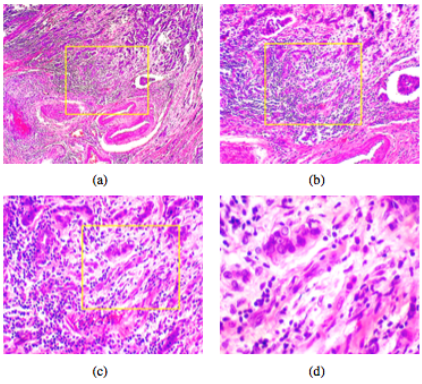
\includegraphics[width=0.8\textwidth]{logo.png}\par\vspace{1cm} % Imagen más grande
    {\scshape\Large Realizado por:\par}
    \vspace{1cm}
    {\Large \theauthor\par}
    \vfill
    {\large \thedate\par}
\end{titlepage}

% RESUMEN
\section*{Resumen}
Este proyecto se enmarca en la asignatura de Procesamiento de Imágenes Digitales (PID) y tiene como objetivo desarrollar un sistema que detecte el cáncer de mama mediante la identificación y comparación de células cancerígenas con células sanas. La metodología se basará en el uso de redes neuronales convolucionales (CNN) para analizar imágenes digitales de tejido mamario y extraer patrones característicos. Se realizan procesos de preprocesamiento y segmentación para aislar las áreas de interés, seguidos de la extracción de características específicas que permitan distinguir entre células malignas y benignas. Con este enfoque, se busca crear una herramienta de apoyo al diagnóstico clínico, que contribuya a una detección temprana y más precisa de la enfermedad.

\vspace{.5cm}

\textbf{Palabras clave:} cáncer de mama, redes neuronales convolucionales (CNN), células, benigno, maligno.

\newpage
% ÍNDICE
\tableofcontents

\newpage

% CONTENIDO
\section{Introducción}
El cáncer de mama es una de las principales causas de mortalidad en el mundo, habiendo sido la responsable de 670.000 muertes en 2022 siendo a su vez el tipo de cáncer más común en las mujeres según \cite{who_breast_cancer}. Esto provoca que durante los últimos años se haya estado realizando una labor social enorme referente a la concienciación sobre el cáncer de mama dando gran importancia a su pronta detección.\\

Gracias a los avances en Deep Learning \cite{shinde2018review}, se han desarrollado métodos innovadores para analizar imágenes histológicas y detectar el cáncer de mama. En este contexto, existen dos aproximaciones que se han estudiado en la literatura, como en el artículo textbf{“Classification of breast cancer based on histology images using convolutional neural networks}” \cite{bardou2018classification}, soportada por los 445 artículos en los que se realiza un estudio entre dos enfoques.\\

Este proyecto tiene como objetivo el desarrollo de una aplicación capaz de detectar cáncer de mama a partir de imágenes histológicas, utilizando dos enfoques complementarios. El primero se basa en una red neuronal convolucional (CNN) que realiza clasificación directamente a la imagen, y un segundo enfoque, basado en extracción de características seguida de la clasificación mediante el algoritmo K-Nearest Neighbors (KNN).\\

El enfoque basado en KNN está inspirado en el trabajo de \cite{bardou2018classification}, quienes proponen una combinación entre la codificación de características visuales utilizando técnicas como -bag of words y locality-constrained linear coding— y clasificadores tradicionales. En su estudio, se demostró que la extracción estructurada de características, combinada con métodos como KNN, puede lograr resultados competitivos en la clasificación de imágenes histológicas de cáncer de mama.\\

Por otro lado, el segundo enfoque se fundamenta en redes neuronales convolucionales, que han mostrado gran efectividad en la clasificación automática de imágenes biomédicas. Específicamente, el trabajo de \cite{minarno2021cnn} implementa un autoencoder basado en CNN para la recuperación de imágenes de cáncer de mama, permitiendo identificar imágenes similares dentro de grandes bases de datos. Esta capacidad de aprendizaje profundo permite al modelo extraer representaciones jerárquicas y semánticas directamente desde los datos crudos, sin necesidad de ingeniería manual de características.\\

Este último aprovecha la potencia de las Redes Neuronales Convolucionales (CNN), un tipo de red neuronal feedforward inspirada en la percepción visual \cite{hubel1962receptive}. Las CNN aplican filtros o “kernels” a lo largo de las imágenes para extraer automáticamente patrones y características como bordes, texturas y formas. Esta capacidad de aprender de forma automática elimina la necesidad de una extracción manual de atributos y, al reducir significativamente el número de conexiones en comparación con una red completamente conectada (FC), permite una convergencia más rápida y una actualización de pesos más eficiente durante el entrenamiento (véase Fig. \ref{fig:capas_convolucionales} Capas convolucionales).\\
\begin{figure}[!ht]
    \centering
    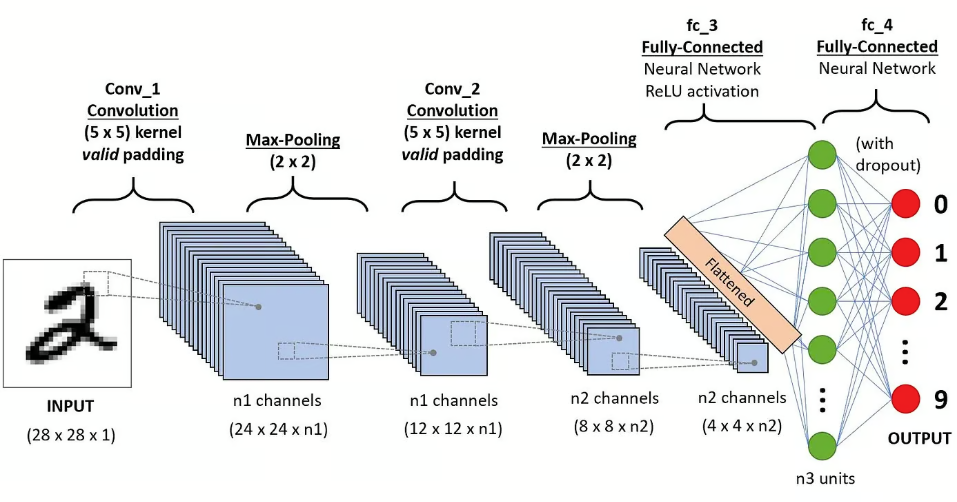
\includegraphics[width=0.8\textwidth]{CNN.png}
    \caption{Capas convolucionales \cite{datacamp_cnn}}
    \label{fig:capas_convolucionales}
\end{figure}\\

\newpage
Ambos enfoques son implementados y evaluados en este proyecto, comparando su rendimiento y su viabilidad para una futura aplicación en el diagnóstico asistido por computadora.\\

El objetivo de este proyecto es desarrollar un sistema que permita detectar el cáncer de mama a partir de imágenes histológicas, utilizando técnicas de aprendizaje automático y redes neuronales convolucionales. Se espera que este sistema contribuya a la mejora en la detección temprana del cáncer de mama, facilitando el trabajo de los profesionales médicos y aumentando la tasa de supervivencia de las pacientes.

El objetivo de nuestro trabajo es desarrollar una red convolucional capaz de detectar el cáncer de mama a partir de imágenes histológicas obtenidas de un dataset público \cite{nasser2023deep} y comparar distintas aproximaciones para evaluar la eficacia en la detección temprana de esta enfermedad.

\newpage
\section{Planteamiento del Teórico}
\subsection{Objetivos del Proyecto}
Este trabajo tiene como objetivo principal analizar y comparar diferentes metodologías de clasificación de imágenes médicas, con especial atención en la detección temprana del cáncer de mama. Para ello, se estudian tanto enfoques tradicionales de clasificación basados en extracción manual de características como enfoques modernos basados en aprendizaje profundo. Los objetivos específicos del proyecto son los siguientes:\\


\begin{enumerate}
    \item \textbf{Crear} una aplicacion que permita a los médicos detectar el cancer de mama solo dando la imagen.
    \item \textbf{Desarrollar} distintos modelos que permitan la clasificacion binaria de las imagenes.
    \item \textbf{Evaluar} el rendimiento de distintos modelos, tanto CNN en tareas de clasificación binaria como KNN.
    \item \textbf{Realizar experimentación para análisis} del  impacto de las técnicas de aumento de datos sobre el desempeño de los modelos.

\end{enumerate}
\subsection{Tecnologías Utilizadas}
Para el desarrollo del proyecto se ha utilizado el lenguaje de programación \textbf{Python}, ampliamente adoptado en la comunidad científica por su simplicidad, legibilidad y amplio ecosistema de bibliotecas para el análisis de datos, visión por computador y aprendizaje automático.\\

Entre estas bibliotecas, se ha seleccionado \textbf{TensorFlow} como herramienta principal para la implementación y comparación de modelos. TensorFlow es una librería de código abierto desarrollada por Google que permite construir, entrenar y desplegar modelos de \textit{machine learning}, especialmente redes neuronales profundas. Su flexibilidad y eficiencia lo convierten en una plataforma ideal tanto para métodos tradicionales como para arquitecturas más complejas basadas en aprendizaje profundo.\\

\subsubsection{Enfoque 1: Redes Neuronales Convolucionales (CNN)}
Una \textbf{Red Neuronal Convolucional} (CNN, por sus siglas en inglés) es un tipo de arquitectura de red neuronal especializada en procesar datos con una estructura de tipo cuadrícula, como las imágenes. Su principal fortaleza radica en su capacidad para aprender representaciones espaciales jerárquicas mediante capas convolucionales.\\

\textbf{Estructura típica de una CNN:}
\begin{enumerate}
    \item \textbf{Capa Convolucional (Convolutional Layer):} Esta capa aplica filtros (o kernels) sobre la imagen de entrada para extraer características locales, como bordes, texturas o patrones específicos. El proceso de convolución genera mapas de activación que representan la presencia de ciertas características.
    \item \textbf{Función de Activación (ReLU):} Tras cada convolución, se aplica normalmente una función de activación como ReLU (Rectified Linear Unit) para introducir no linealidades, lo que permite a la red aprender funciones más complejas.
    \item \textbf{Capa de Agrupamiento (Pooling Layer):} Reduce la dimensionalidad de los mapas de activación, conservando las características más relevantes. El tipo más común es \textit{max pooling}, que selecciona el valor máximo en regiones locales.
    \item \textbf{Capas Completamente Conectadas (Fully Connected Layers):} Al final de la red, estas capas interpretan las características extraídas para realizar la predicción final, como clasificar si una imagen muestra tejido sano o indicios de cáncer.
    \item \textbf{Capa de Salida:} Generalmente una capa \textit{softmax} (para clasificación multiclase) o una sigmoide (para clasificación binaria), que devuelve la probabilidad de pertenencia a cada clase.

\end{enumerate}

Las CNN se entrenan mediante retropropagación (backpropagation) y optimización mediante algoritmos como Adam o SGD, ajustando los pesos para minimizar una función de pérdida, habitualmente la entropía cruzada (\textit{binary cross-entropy} en problemas binarios).

\subsubsection{Enfoque 2: Autoencoder y KNN sobre la Capa Latente}
Un \textbf{autoencoder} es una red neuronal no supervisada diseñada para aprender una representación comprimida (latente) de los datos, útil para tareas como reducción de dimensionalidad, eliminación de ruido o extracción de características.

\textbf{Estructura de un autoencoder:}
\begin{enumerate}
    \item \textbf{Codificador (Encoder):} Esta parte reduce progresivamente la dimensión de la entrada, transformándola en una representación más compacta. Se compone de varias capas densas o convolucionales, según el tipo de dato.
    \item \textbf{Capa Latente (Bottleneck):} Es la representación más comprimida de la entrada. Idealmente, contiene la información esencial del patrón original y descarta el ruido o redundancias. Esta es la capa que se utilizará para aplicar métodos de clasificación tradicionales, como KNN.
    \item \textbf{Decodificador (Decoder):} Reconstruye la entrada original a partir de la capa latente, tratando de minimizar la diferencia entre entrada y salida (p. ej., usando el error cuadrático medio como función de pérdida).
\end{enumerate}

Una vez entrenado el autoencoder, se prescinde del decodificador y se conserva únicamente el \textbf{codificador}, que transforma las imágenes en vectores de baja dimensión. Sobre estos vectores comprimidos se aplica el algoritmo \textbf{K-Nearest Neighbors (KNN)}, que clasifica nuevas imágenes comparándolas con las más cercanas en el espacio latente. Esta estrategia permite combinar lo mejor de ambos mundos: una representación no lineal potente (extraída por el autoencoder) y un clasificador sencillo, interpretable y eficaz como KNN.\\

En concreto, en este proyecto, el modelo CNN ya se encontraba predefinido en el articulo \cite{bardou2018classification}, por lo que solo ha sido necesario construir la red neuronal la cual ha sido entrenada con el dataset \textbf{BreakHis}, en concreto se han generado 5 modelos, uno entrenado con el datase completo y uno generado por cada magnificación disponible del dataset (40X, 100X, 200X, 400X), por otra parte, el modelo KNN, se divide en dos partes, la extraccion de características y la clasificacion, la extraccion de características se ha obtenido a partir del autoencoder descrito en el articulo \cite{minarno2021cnn} y el clasificador KNN realizado manualmente.

\newpage
\section{Implementación}
El desarrollo de este proyecto se fundamenta en el uso de técnicas de aprendizaje automático y profundo para la clasificación de imágenes histológicas de cáncer de mama. Con el objetivo de comparar el rendimiento entre distintos enfoques, se han implementado y entrenado dos tipos de modelos: uno basado en un clasificador K-Nearest Neighbors (KNN) acompañado de un proceso de extracción de características, y otro basado en una red neuronal convolucional (CNN). Ambos modelos han sido entrenados utilizando un conjunto de imágenes histológicas públicamente disponible, asociado al trabajo de Bardou et al. [1]. Este dataset incluye imágenes con diferentes niveles de magnificación (40x, 100x, 200x y 400x), aunque el artículo original no proporciona demasiados detalles sobre la obtención de las imágenes ni sobre las características clínicas asociadas.\\

\subsection{Descripción del dataset}
Para el desarrollo de este proyecto se utilizó el \textbf{dataset de imágenes histológicas de cáncer de mama BreaKHis} \cite{google_drive_folder}, asociado al trabajo de \cite{bardou2018classification}. Este conjunto de datos es ampliamente utilizado en la literatura científica para la investigación en diagnóstico asistido por computadora en cáncer de mama. BreaKHis contiene \textbf{7909 imágenes histológicas} de biopsias mamarias, distribuidas en dos clases principales: \textbf{benignas} y \textbf{malignas}, en concreto, \textbf{2480 imágenes benignas}, subdivididas en cuatro subtipos: adenosis, fibroadenoma, tumor filoides y tejido conectivo y  \textbf{5429 imágenes malignas}, subdivididas en carcinoma ductal, carcinoma lobulillar, carcinoma mucinoso y carcinoma papilar. Las imágenes fueron adquiridas a partir de muestras teñidas con hematoxilina y eosina \texttt{(H\&E)} y capturadas con un microscopio óptico en diferentes niveles de aumento: \textbf{40x, 100x, 200x y 400x}.\\

Las imágenes tienen una resolución de 700×460 píxeles en formato PNG y están organizadas por paciente, clase y magnificación. Una característica importante del dataset es que mantiene la trazabilidad del origen de las imágenes (es decir, a qué paciente pertenecen), lo que permite realizar particiones de entrenamiento y prueba sin mezclar muestras del mismo paciente entre ambos conjuntos, reduciendo así el riesgo de sobreajuste.

\subsection{Arquitectura de la aplicación}
La aplicación desarrollada para el análisis de cáncer de mama mediante modelos KNN y CNN ofrece una interfaz gráfica intuitiva basada en Tkinter, que permite al usuario interactuar fácilmente con el sistema. Una de sus funcionalidades principales es la carga de imágenes, donde el usuario puede seleccionar desde su dispositivo una imagen médica, la cual se muestra en una vista previa dentro de la interfaz para su verificación.\\

Además, la aplicación permite la selección de distintos modelos preentrenados, tanto de tipo KNN (como “KNN(all)” o “KNN(aux)”) como de redes neuronales convolucionales (CNN), con distintas configuraciones que ofrecen flexibilidad en el análisis. Esta selección de modelo es esencial para personalizar el tipo de procesamiento que se aplicará sobre la imagen cargada.\\

Una vez seleccionados la imagen y el modelo, el usuario puede iniciar el análisis pulsando un botón. El sistema entonces ejecuta el modelo correspondiente, determinando si el caso es benigno o maligno. El resultado se muestra de forma clara mediante un mensaje textual, un icono visual asociado al diagnóstico, y un conjunto de estadísticas adicionales que aportan más contexto al resultado obtenido.\\

La aplicación también gestiona de forma inteligente el estado de la interfaz: desactiva el botón de análisis si no se han cumplido los requisitos previos (imagen y modelo seleccionados), y limpia automáticamente los resultados anteriores cuando se cargan nuevos datos. Gracias a su diseño estructurado y al uso de componentes \textit{ttk}, la experiencia del usuario es fluida y profesional, facilitando la interpretación del diagnóstico por parte de usuarios tanto técnicos como clínicos.\\

\subsubsection{Arquitectura CNN}
En el ámbito del aprendizaje automático, las redes neuronales convolucionales \texttt{(CNN)} se han convertido en una tendencia dominante, alcanzando un notable éxito en diversas áreas como la visión por computador y el reconocimiento de voz. En este contexto, Bardou, Zhang y Ahmad en \cite{bardou2018classification} proponen una arquitectura CNN específicamente diseñada para la clasificación de imágenes histológicas de cáncer de mama teñidas con hematoxilina y eosina \texttt{(H\&E)}, diferenciando entre tejidos benignos y malignos. La arquitectura fue implementada utilizando el popular framework BVLC Caffe \cite{jia2014caffe}, desarrollado por la Universidad de California, Berkeley. Este entorno permite diseñar e implementar redes CNN de forma sencilla, con interfaces disponibles tanto para \textit{MATLAB} como para Python, y soporte para entrenamiento en CPU y GPU. El modelo CNN propuesto se especifica mediante archivos de configuración que definen la estructura de la red y los parámetros de optimización.\\

La arquitectura propuesta consta de cinco capas convolucionales seguidas por dos capas completamente conectadas y una capa softmax de salida. En detalle, la primera capa convolucional utiliza filtros de tamaño 3×3 y genera 64 mapas de características; la segunda también emplea filtros de 3×3 pero produce 96 mapas; la tercera capa, con filtros del mismo tamaño, genera 128 mapas de características; la cuarta capa incrementa esta cifra a 256 mapas, al igual que la quinta capa. Posteriormente, se añaden dos capas completamente conectadas, la primera con 2000 unidades ocultas y la segunda con tantas unidades como clases tenga el conjunto de datos. Finalmente, una capa softmax se encarga de la clasificación. Todas las capas convolucionales y completamente conectadas aplican la función de activación ReLU \texttt{(Rectified Linear Unit)}, definida como: \begin{equation} f(x) = \max(0, x) \end{equation}lo que introduce no linealidades y acelera la convergencia del entrenamiento.\\

Además, se utiliza max pooling tras las capas convolucionales primera, segunda y quinta. Esta técnica de reducción de dimensión espacial se aplica después de ReLU con un filtro de tamaño 3×3 y un desplazamiento \texttt{(stride)} de 2. Las capas tercera y cuarta no incorporan pooling, probablemente para preservar la resolución espacial de las características extraídas. \\

El peso de las capas se inicializa mediante una distribución gaussiana con desviación estándar baja ($0.01$), mientras que la regularización se aborda con varias estrategias. Por un lado, se incluye una capa de \textit{dropout} después de la primera capa completamente conectada, con una probabilidad de retención (\textit{keep probability}) de $\rho = 0.5$, lo cual ayuda a mitigar el sobreajuste. Por otro lado, se aplica una penalización de tipo $L_2$ (\textit{weight decay}) con un valor $\lambda = 10^{-3}$ para restringir los valores de los pesos durante el entrenamiento.\\

El modelo se entrena mediante el algoritmo de descenso de gradiente estocástico (SGD), con un tamaño de lote (\textit{batch size}) igual a 32. La tasa de aprendizaje inicial se establece en $0.001$ y se ajusta dinámicamente durante el entrenamiento utilizando una política de decaimiento inverso cada cinco épocas. Este parámetro controla la magnitud de los pasos que da la red en cada iteración para minimizar la función de pérdida. Además, se incorpora un factor de momento (\textit{momentum}) de $0.9$, que favorece una convergencia más estable y ayuda a evitar quedarse atrapado en mínimos locales. Finalmente, los datos de entrada se barajan aleatoriamente antes de cada época para prevenir sesgos asociados a un orden fijo en el conjunto de entrenamiento.\\

En conjunto, esta arquitectura CNN logra una extracción jerárquica de características efectivas, desde patrones locales hasta representaciones globales, optimizando así el rendimiento en la clasificación de imágenes histológicas. Los resultados reportados demuestran que esta red supera a los métodos clásicos basados en características manuales, lo que refuerza la utilidad de las CNN en aplicaciones de diagnóstico asistido por computadora en el ámbito de la patología digital.\\

\subsubsection{Arquitectura KNN}
El artículo \cite{minarno2021cnn}, propone una metodología innovadora para la extracción automática de características en imágenes histológicas de cáncer de mama, basada en autoencoders convolucionales (CNN-AE). Este enfoque permite representar imágenes complejas en forma de vectores latentes que conservan la información más relevante para tareas posteriores como clasificación o recuperación por similitud. \\

\textbf{Arquitectura del Autoencoder:}
El autoencoder se entrena mediante un proceso iterativo en el que se minimiza la diferencia entre la imagen original y su reconstrucción (error de reconstrucción). Este error se calcula usando una función de pérdida (como el error cuadrático medio), y se optimiza con métodos como el descenso de gradiente estocástico (SGD) o el optimizador Adam. Durante el entrenamiento, se emplea un conjunto de datos dividido en subconjuntos de \textbf{entrenamiento} y \textbf{validación}, lo cual permite evaluar el rendimiento general del modelo y evitar el sobreajuste.\\

De forma específica, el proceso incluye tres pasos fundamentales:\\

\begin{enumerate}
    \item \textbf{Codificación (Encoder):} compresión de la imagen en una representación latente compacta.
    \item \textbf{Decodificación (Decoder):} reconstrucción de la imagen a partir del vector latente.
    \item \textbf{Cálculo de la función de pérdida y optimización:} ajuste iterativo de los pesos para minimizar el error de reconstrucción.
\end{enumerate}

Además, se implementa una política de \textbf{almacenamiento del mejor modelo}, en la cual se guarda la versión del autoencoder que presenta el \textbf{menor valor de pérdida} en el conjunto de validación. Este modelo óptimo se utilizará posteriormente \textbf{para la extracción de características y recuperación de imágenes.}\\


\textbf{Extracción de Características para Recuperación y Clasificación:}

Una vez entrenado, el \textbf{codificador} se desacopla del decodificador y se utiliza de manera independiente para transformar imágenes en vectores latentes. Esta operación consiste en alimentar una imagen al codificador y capturar la activación de su capa más profunda, justo antes de la entrada al decodificador. El vector de salida obtenido en esta etapa representa una \textbf{caracterización compacta} y discriminativa de la imagen de entrada y se conforma de 48 valores, preservando información estructural crucial para la identificación de patrones asociados al cáncer de mama. Estos vectores de características se almacenan en una base de datos y se emplean como entrada para clasificadores como k-NN. En los experimentos realizados, se evaluó la precisión del sistema mediante:

\begin{itemize}
    \item \textbf{Clasificación binaria} (benigno vs. maligno): alcanzando una precisión promedio de \textbf{$92.37\%$}.
\end{itemize}

\textbf{Clasificación mediante k-NN utilizando Vectores Latentes:}

Tras el proceso de extracción de características mediante el autoencoder convolucional, cada imagen del conjunto de datos fue transformada en un vector latente de dimensión reducida, representando las características más relevantes de la imagen histológica. Estos vectores latentes, junto con su etiqueta de clase correspondiente (por ejemplo, benigno o maligno), fueron almacenados en un archivo \textbf{JSON}, actuando como base de datos para el sistema de clasificación.\\

Para realizar la clasificación de una nueva imagen, se sigue el siguiente procedimiento:

\begin{enumerate}
    \item \textbf{Extracción del vector latente:} La imagen de entrada se procesa a través del codificador previamente entrenado, obteniendo su correspondiente vector de características.
    
    \item \textbf{Cálculo de distancias:} Se calcula la \textbf{distancia euclídea} entre el vector extraído de la imagen a predecir y todos los vectores almacenados en el archivo JSON. La distancia euclídea entre dos vectores \( x \) e \( y \) se define como:
    
    \begin{equation}
        d(x, y) = \sqrt{ \sum_{i=1} (x_i - y_i)^2 }
    \end{equation}

    \item \textbf{Selección de los vecinos más cercanos:} Una vez calculadas todas las distancias, se seleccionan los \textbf{k vectores más cercanos}, siendo \(k \)= 5 en esta implementación. Estos representan las imágenes más similares en el espacio latente.
    \item \textbf{Clasificación por mayoría:} Se toma la clase más común entre los cinco vectores más próximos, y esta se asigna como la \textbf{predicción final} para la imagen de entrada.

\end{enumerate}

Este enfoque no requiere un entrenamiento explícito del clasificador, ya que el método k-NN funciona de forma \textbf{perezosa} (lazy learning), basándose directamente en las instancias almacenadas y las comparaciones entre vectores. Gracias a la alta calidad de las características extraídas por el autoencoder, el sistema logra clasificaciones precisas sin necesidad de arquitecturas más complejas.

\subsection{Evaluación del Sistema}
Los modelos fueron evaluados mediante un conjunto de métricas de clasificación binaria:

\begin{enumerate}
    \item \textbf{Precisión (accuracy):} mide la proporción de predicciones correctas respecto al total de muestras evaluadas. Se calcula como:
    \begin{equation}
        \text{acc} = \frac{VP + VN}{n} = \frac{R_v}{n}
    \end{equation}
    \item \textbf{Sensibilidad (recall):} evalúa la capacidad del modelo para identificar correctamente las muestras positivas. Se calcula como:
    \begin{equation}
        \text{recall } = \frac{R_v}{M}
    \end{equation}
    \item \textbf{Especificidad:} cuantifica la proporción de muestras negativas que fueron correctamente clasificadas. Scalcula como:
    \begin{equation}
        \text{prec} = \frac{VN}{VN + FP}
    \end{equation}
    \item \textbf{F1 Score:} proporciona una medida balanceada entre la precisión y la sensibilidad, siendo especialmente útil en contextos donde existe un desequilibrio entre clases. Se calcula como:
    \begin{equation}
        F1 = 2 \cdot \frac{\text{prec} \cdot \text{recall}}{\text{prec} + \text{recall}}
    \end{equation}
\end{enumerate}

Estas métricas fueron calculadas de forma individual para cada uno de los modelos entrenados, lo que permitió realizar un análisis cuantitativo del impacto que tiene el tipo de arquitectura como \textit{K-Nearest Neighbors} (KNN) y \textit{Convolutional Neural Networks} (CNN) sobre el rendimiento en la tarea de clasificación. \\

Adicionalmente, se evaluó la influencia de distintos niveles de \textit{data augmentation} aplicados a las imágenes de entrada, con el fin de observar cómo afectan la capacidad de generalización de los modelos.\\

Además, se llevó a cabo un análisis de robustez para estudiar el comportamiento de los modelos ante variaciones morfológicas y diferencias en la resolución entre las imágenes. Esta evaluación buscó determinar en qué medida los modelos eran capaces de mantener un rendimiento aceptable frente a datos que presentan una alta variabilidad estructural, un aspecto crucial en contextos donde los datos de entrada no son homogéneos ni ideales.

\section{Experimentación}
Para llevar a cabo la experimentación, se realizaron pruebas sobre un conjunto de datos al que se le aplicará \textit{data augmentation} con el objetivo de evaluar la robustez y capacidad de generalización de los modelos. Las técnicas de aumento de datos incluirán transformaciones como rotaciones de un rango entre $-30^\circ$ a $30^\circ$ y modificaciones en la intensidad de las imágenes, con un factor de entre $0.7$ (oscurece) a $1.3$ (ilumina), simulando variaciones realistas que podrían encontrarse en escenarios del mundo real. Esto permitirá analizar cómo afecta la variabilidad de entrada al rendimiento de los modelos evaluados. \\

En esta etapa, se llevará a cabo una comparación de rendimiento entre dos enfoques de clasificación: una red neuronal convolucional (\textit{CNN}) entrenada sobre cada variedad de las imágenes aumentadas y un entrenamiento con todas las imágenes en global, y un modelo \textit{K-Nearest Neighbors} (\textit{KNN}) diseñado de forma personalizada para cada uno de las posibles variaciones de imágenes respecto a su aumento. Esta comparación permitirá observar las diferencias entre un enfoque basado en aprendizaje profundo y otro basado en métodos clásicos de aprendizaje supervisado, en cuanto a métricas de \textit{precisión}, \textit{recall} y \textit{F1-score}.

% TODO: meter comparaciones de características


\section{Manual de usuario}
Aquí van las conclusiones.

\section{Conclusiones}
Aquí van las conclusiones.

\section{Autoevaluación de cada miembro del equipo}
Aquí van las conclusiones.

\section{Tabla de tiempos}
Aquí van las conclusiones.

\addcontentsline{toc}{section}{Bibliografía} 
\printbibliography

\end{document}
